Este capítulo aborda a base teórica necessária para o desenvolvimento do projeto.

\section{Arquitetura RISC-V: ISA}

	Sua arquitetura obedece aos padrões RISC (Reduced Instruction Set Computing), tendo instruções simples e completas. Foi projetada para ser rápida, ocupar pouco espaço físico, ter baixo consumo de energia, ser extensível, e compatível com entre suas versões. Por ser reduzida, se encaixa perfeitamente para fins acadêmicos, e pesquisas. 

	Outra característica importante é a sua extensibilidade. Por padrão sua base é inteira, para arquiteturas de 32, 64 e 128 bits, porém existem módulos de extensão. Para descrever quais implementações são utilizadas utilizam-se as nomenclaturas RV32I, RV64I e RV128I, para as implementações padrões RISC-V 32 bits, 64, e 128.

	Existem módulos padrões e não-padrões de extensões~\cite{riscv_spec}:

		\begin{itemize}
			\item Os módulos padrões são aqueles que não possuem conflitos entre si e são utizados para propósitos gerais.
			\item Os módulos não-padrões são módulos especializados, podendo conflitar com outros módulos. A previsão é de que no futuro hajam muitos módulos desse tipo.
		\end{itemize}

	Os padrões desenvolvidos atualmente adicionam as letras "IMAFDQLCBJTPVN", sendo que cada letra representa uma extensão

		\begin{itemize}
			\item I: Integer
			\item M: Multiply/Divide
			\item A: Atomic
			\item F: Single-Precision Floating-Point
			\item D: Double-Precision Floating-Point
			\item Q: Quad-Precision Floating-Point
			\item L: Decimal Floating-Point
			\item C: 16-bit Compressed Instructions
			\item B: Bit Manipulation
			\item J: Dynamic Languages
			\item T: Transactional Memory
			\item P: Packed-SIMD Extensions
			\item V: Vector Extensions 
			\item N: User-Level Interrupts 
		\end{itemize}

	As extensões IMAFD são chamadas de extensões de propósito geral e são abreviadas por G, por exemplo, uma arquitetura de 32 bits que utilizam todas as extensões de propósito geral é chamada de RV32G.

	Ainda existe uma outra variação que é a extensão "E", que se difere das outras pois é projetada para sistemas embarcados. Este módulo diminui a quantidade de registradores para 16 e o tamanho também é reduzido para 16 bits.

	\subsection{Objetivos}

		Seus projetistas sempre são perguntados o motivo ao qual eles quiseram desenvolver uma nova ISA. Alguns dos motivos para o qual usar uma ISA comercial são: a existência de suporte de um ecossistema de software, incluindo ferramentas de desenvolvimento, portabilidade e ferramentas educacionais; a grande quantidade de documentação; tutoriais e exemplos para o desenvolvimento.

		Porém estas vantagens são pequenas na prática, e listam várias disvantagens ao utilizar ISAs comerciais,

		\begin{itemize}
			\item ISAs comerciais são proprietárias
			\item ISAs comerciais são populares somente em alguns nichos do mercado
			\item ISAs comerciais vem e vão
			\item ISAs populares são complexas
			\item ISAs comerciais dependem de outros fatores para trazer aplicações
			\item ISAs comerciais populares não são projetadas para extensibilidade
			\item Uma ISA comercial modificada é uma nova ISA
		\end{itemize}

		Na opinião dos projetistas do RISC-V, em um sistema computacional, a ISA é a interface mais importante, e não existe razão pra que esta seja proprietária~\cite{Waterman:EECS-2016-1}. E uma ISA livre e aberta tem um potencial de inovação, redução de custos muito maior. 

		A ISA RISC-V tem o propósito de uso geral, ou seja, você pode implementar esta arquitetura para uma variedade de problemas, desde Internet das coisas até aplicações de alta performance. Para isso os projetistas tiveram a preocupação de fornecer uma ISA o mais simples possível e modular, portanto para resolver tipos diferentes de problemas se pode utilizar módulos diferentes já citados anteriormente neste capítulo.

	\subsection{História}%
		A ISA RISC-V foi originalmente desenvolvida na Universidade da Califórnia, Berkeley, na Divisão de Ciência da computação, no departamento de Engenharia Elétrica e Ciência da Computação. Baseada na experiência com projetos passados de seus projetistas, a definição da ISA foi iniciada no verão de 2010.\

		Em 13 de maio de 2011, foi lançada a primeira documentação para nível de usuário, \textit{The RISC-V Instruction Set Manual, Volume I: Base User-Level ISA} ~\cite{riscv_manual_v1}

		Em 6 de maio de 2014, saiu a versão 2.0 do manual, \textit{The RISC-V Instruction Set Manual, Volume I: Base User-Level ISA, Version 2.0} ~\cite{riscv_manual_v2}

		Em 7 de maio de 2017, a versão 2.2 que utilizamos neste projeto foi lançada, \textit{The RISC-V Instruction Set ManualVolume I: User-Level ISA Document Version 2.2}~\cite{riscv_spec}.

		Os primeiros processadores RISC-V fabricados foram escritos em Verilog e manufaturados em tecnologia de pré-produção de 28 nm FD-SOI (\textit{Fully Depleted Silicon On Insulator}) da companhia STMicroeletronics com o nome \textit{Raven-1} em maio de 2011.

		As últimas implementações fabricadas documentadas no manual são os processadores EOS22 em março de 2014, pela IBM usando a tecnologia 45nm SOI.

		A ISA tem sido utilizada em cursos de Universidade da Califórnia em Berkeley desde 2011.

		%Andrew Waterman and Yunsup Lee developed the C++ ISA simulator “Spike”, used as a golden model in development and named after the golden spike used to celebrate completion of the US transcontinental railway. Spike has been made available as a BSD open-source project.

	

	\subsection{RISC-V Foundation}
		
		A \textit{RISC-V Foundation} é uma organização sem fins lucrativos, criada para direcionar futuro desenvolvimento e incentivar a utilização da ISA RISC-V.\ ~\cite{riscv_foundation} 

		O presidente do conselho atualmente é Krste Asanovic, professor do departamento de Engenharia elétrica e ciência da computação na Universidade da Califórnia em Berkeley. Ele é também co-fundador da empresa SiFive Inc., a qual incentiva do uso comercial de processadores RISC-V.\

		O vice-presidente da RISC-V Foundation é o professor David Patterson, muito conhecido pelo livro \textit{Computer Architecture: A Quantitative Approach}, que escreveu juntamente com John Hennessy, e suas pesquisas relacionadas a RISC, RAID, e Redes de estações de trabalho.\

		Outros membros incluem:\
		\begin{itemize}  
			\item Zvonimir Bandic, pesquisador e diretor da Western Digital Corporation. 
			\item Charlie Hauck, CEO da Bluespec Inc.
			\item Frans Sijstermans, vice presidente de engenharia da NVIDIA.
			\item Ted Speers, chefe de arquitetura de produtos e planejamento do grupo SoC da Microsemi.
			\item Rob Oshana, gerente de desenvolvimento de software e negócios em segurança na NXP Semiconductors. 
		\end{itemize}

		e também, Sue Leininger, gerente de comunidade e Rick O’Connor, director executivo.~\cite{riscv_fboardmembers}

	\subsection{Open Source}
		
		O modelo de licenciamento que RISC-V utiliza é a \textit{BSD Open Source License}. Ou seja, em caso de utilização, apenas dar créditos aos autores, no caso a UC Berkeley.~\cite{riscv_faq}

		O fato da ISA ser Open Source traz grandes vantagens, principalmente com relação à distribuição e ao compartilhamento.
		
		No aspecto comercial, por exemplo, qualquer pessoa pode criar suas implementações da ISA para seus objetivos específicos e comercializá-las, com seu código fonte podendo ser aberto ou fechado.

		É requisitado, apenas, pela licença, que os autores sejam reconhecidos. Esse modelo contribui para a diminuição dos custos devido ao uso de patentes, e também custos de desenvolvimento pelo reaproveitamento de código.

		Outra vantagem, defendida pelos autores e também defendida no mundo do software livre, é a questão de vulnerabilidades na solução. Apesar de parecer contra intuitivo, o fato do código ser aberto, contribui para que as vulnerabilidades possam 	ser encontradas e consertadas com maior rapidez, sendo dispensável um auditor para lidar com vulnerabilidades implantadas por desenvolvedores maliciosos de dentro da própria empresa. Mesmo que as vulnerabilidades não tenham sido implantadas de forma maliciosa, bugs acontecem e o fato do código ser fechado pode fazer com que esta fique escondida por algum tempo antes de poder ser descoberta e explorada, como foi o caso das vulnerabilidades \textit{Spectre} e \textit{Meltdown}~\cite{meltdown_spectre_exploits} que ganharam atenção na mídia recentemente e estão diretamente ligados ao mundo dos processadores por explorarem vulnerabilidades arquiteturais~\cite{meltdown_spectre_media}.

		A RISC-V Foundation escreveu em seu site oficial que não foram encontrados impactos das vulnerabiliaddes \textit{Meltdown} e \textit{Spectre} em nenhuma implementação até janeiro de 2018. Apesar dos ataques não serem específicos de uma ISA ou outra, mostra uma vantagem de se ter uma ISA aberta, a velocidade de se corrigir os erros pela comunidade é muito maior. E a possibilidade de poder experimentar e testar novas formas eficientes para resolver estes problemas é histórica. ~\cite{riscv_security}.

	\subsection{Modelo de memória}
	
		O espaço de endereços do RISC-V é endereçado byte a byte, na convenção de ordenação \textit{little-endian}. Diferente de arquiteturas como x86 ou ARM, RISC-V utiliza somente endereçamento base+offset com imediato de 12 bits. Pela especificação todos os \textit{loads} e \textit{stores} são desalinhados, porém como é feito varia de implementação pra implementação. A ISA contém a instrução FENCE para ordenação explícita em \textit{threads} e outras sincronizações.

	\subsection{Instruções}

		A ISA básica, ou seja o RV32I, possui quarenta e sete instruções, sendo possível reduzir para trinta e oito com implementações mais simples, descartando algumas instruções de chamadas de sistemas, e de controle de estado de registradores, ou sincronização de memória para recurso de \textit{threading}, substituindo por uma instrução SYSTEM geral, ou substituindo por NOPs.
	
		Existem seis tipos de instruções básicas, como mostradas na figura \ref{fig:instruction_formats},

		\begin{figure}[h]
		  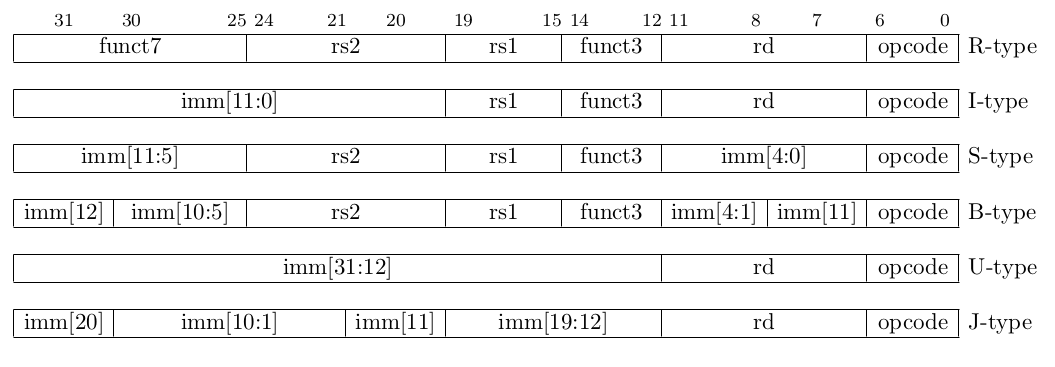
\includegraphics[width=\linewidth]{img/instruction_formats.png}
		  \caption{Formatos de instruções da ISA básica}
		  Fonte: The RISC-V Instruction Set Manual, Volume I: User-Level ISA, Document Version 2.2~\cite{riscv_spec}
		  \label{fig:instruction_formats}
		\end{figure}

		sendo as instruções do tipo B uma variação do tipo S, e as instruções do tipo J uma variação do tipo U. Algumas convenções adotadas são, as posições dos registradores \textit{source} rs1, e rs2, e o registrador de destino rd, sempre ocupam o mesmo lugar nos diferentes formatos, pois isso simplifica a decodificação, além disso, todos os imediatos são extendidos pelo sinal, exceto pelos imediatos das instruções de CSR(\textit{"Control and Status Registers"}). 

		A figura \ref{fig:immediate_encoding}, mostra os imediatos produzidos por cada tipo de intrução e de qual parte da instrução vem cada bit do imediato.

		\begin{figure}[h]
		  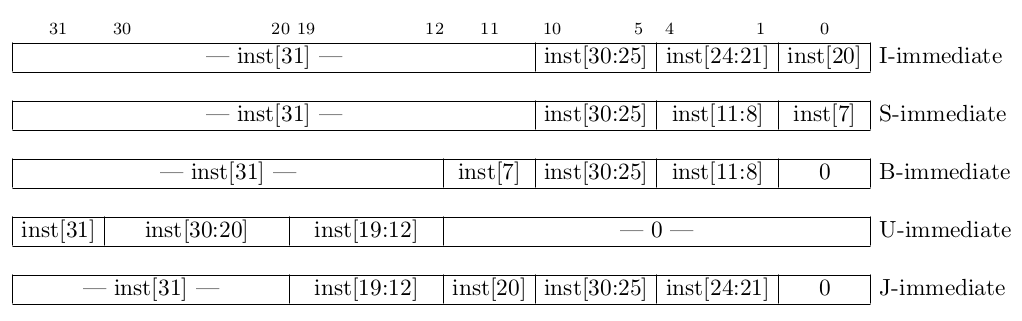
\includegraphics[width=\linewidth]{img/immediate_encoding.png}
		  \caption{Encoding dos imediatos de cada tipo de instrução}
		  Fonte: The RISC-V Instruction Set Manual, Volume I: User-Level ISA, Document Version 2.2~\cite{riscv_spec}
		  \label{fig:immediate_encoding}
		\end{figure}

		As instruções do tipo R, são as do tipo registrador-registrador, utilizam três registradores como argumentos, dois sendo fonte e um de destino por exemplo:
		\begin{itemize}
			\item{ADD x1, x2, x3. Soma os valores do conteúdos nos registradores x2 e x3 e armazena em x1.}
			\item{SUB x1, x2, x3. Subtrai os valores do conteúdos nos registradores x2 e x3 e armazena em x1.}
			\item{XOR x1, x2, x3. Realiza a operação binária XOR dos conteúdos dos registradores x2 e x3 e armazena o resultado em x1.}
			\item{SLT x1, x2, x3. Set Less Than. Insere o valor 1 no registrador x1, se o conteúdo de x2 for menor que o conteúdo de x3, considerando o sinal. Caso contrário, insere o valor 0 em x1.}
			\item{SLL x1, x2, x3. Shift Left Logical. Armazena em x1 o valor de x2 deslocado para esquerda do valor dos cinco bits mais baixos de x3.}				
		\end{itemize}
		Outras instruções incluem, AND, OR, SLTU, SRL, SRA...

		As do tipo I, são as do tipo registrador-imediato, são muito parecidas com as do tipo R porém utilizam um valor explícito do código ao invés de um registrador como um dos argumentos, exemplos:
		\begin{itemize}
			\item{ADDI x1, x2, imm. Soma o valor contido no registrador x2 e imm e armazena em x1.}
			\item{SUBI x1, x2, imm. Subtrai o valor de imm do conteúdo do registradores x2 e armazena em x1.}
			\item{XORI x1, x2, imm. Realiza a operação binária XOR dos conteúdos dos registradores x2 e imm e armazena o resultado em x1.}
			\item{SLTI x1, x2, imm. Set Less Than Immediate. Insere o valor 1 no registrador x1, se o conteúdo de x2 for menor que o valor imm, considerando o sinal. Caso contrário, insere o valor 0 em x1.}
			\item{SLLI x1, x2, imm. Shift Left Logical Immediate. Armazena em x1 o valor de x2 deslocado para esquerda do valor imm.}
		\end{itemize}
		Outras instruções incluem, ANDI, ORI, SLTUI, SRLI, SRAI, e também as instruções de LOAD, e JALR (\textit{"Jump And Link to Register"}).

		As instruções do tipo S são dedicadas as operações de STORE, ou seja, armazenar informações na memória,
		\begin{itemize}
			\item{SB x1, x2, imm. Store Byte. Armazena o byte menos significativo contido em x2 no endereço que se da pelo conteúdo de x1 mais o imm}
			\item{SH x1, x2, imm. Store Halfword. Armazena a halfword menos significativa contida em x2 no endereço que se da pelo conteúdo de x1 mais o imm}
			\item{SW x1, x2, imm. Store Word. Armazena a word contida em x2 no endereço que se da pelo conteúdo de x1 mais o imm.}
		\end{itemize}

		As instruções do tipo B são utilizadas nas operações de BRANCH, ou seja, saltos condicionais,
		\begin{itemize}
			\item{BEQ x1, x2, label , Branch EQual. Se os registradores x1 e x2 tiverem o mesmo conteúdo, o salto é realizado}
			\item{BLT x1, x2, label , Branch Less Than. Se o valor de x1 for menor que o de x2, o salto é realizado}
			\item{BLTU x1, x2, label , Branch Less Than Unsigned. Se o valor inteiro sem sinal de x1 for menor que x2 o salto é realizado }
		\end{itemize}

		As instruções do tipo U são utilizadas nas operações LUI e AUIPC,
		\begin{itemize}
			\item{Load Upper Immediate, LUI x1, imm. Carrega os 20 bits de imediato nos 20 bits mais significativos de x1 e completa com zeros}
			\item{Add Upper Immediate to PC, AUIPC. Adiciona 12 bits zerados aos 20 bits do imediato e soma ao valor do contador de programa.}
		\end{itemize}

		E finalmente a instrução tipo J para saltos incondicionais, 
		\begin{itemize}
			\item{JAL x1, addr. Jump And Link. Salva o valor de PC+4 em x1 e salta para o valor de PC+addr}
		\end{itemize}


\section{Montador}

	Um montador é basicamente um software que traduz um programa-fonte em linguagem de máquina. O montador traduz códigos da linguagem \textit{Assembly}, e é um passo intermediário entre a compilação de um código em linguagem de alto nível como \textit{C/C++}, \textit{Java}, \textit{Fortran} para linguagem de máquina.

	\subsection{Algoritmo de duas passagens}

		O algoritmo utilizado para a implementação do montador se chama Algoritmo de duas passagens, esse nome é devido ao fato de que dado o código fonte da aplicação precisa ser ser lido pelo algoritmo duas vezes para poder realizar a montagem completa. É o algoritmo mais simples de ser implementado e tem grande eficiência. O algoritmo de uma passagem é mais rápido porém consome mais memória, além de outros detalhes. 

		O processo de montagem pode ser dividido em quatro partes dentro do algoritmo,

		\begin{itemize}
			\item Análise Léxica, esta parte do código é responsável por limpar o código o máximo possível, retirando todo tipo de informação desnecessária como por exemplo, espaços em branco, tabulações, e comentários. No processo é criado grupo de tokens.
			\item Análise Sintática, também conhecido como \textit{parser} em inglês, faz uma checagem de algumas regras da linguagem, por exemplo uma instrução inexistente sendo utilizada, ou uma diretiva, ou símbolos em lugares indevidos, por exemplo, se ao invés de utilizar vírgulas entre os argumentos de uma instrução, utilizar asteriscos.
			\item Análise Semântica verifica erros que utilizam sintaxes corretas, porém em lugares errados, por exemplo ao tentar utilizar uma instrução ADD com um imediato como argumento, ou então tentar realizar um JUMP para uma label não declarada. 
			\item Geração de código é a parte mais direta, com o auxílio de uma tabela da linguagem, transforma os tokens em código binário com a codificação necessária para o processador saber onde estão as informações necessárias.
		\end{itemize} 


\section{Aplicações web}

	As aplicações web, são aquelas projetadas para que sua utilização seja feita através de um navegador com acesso à Internet.

	\subsection{Arquitetura}
		
		Como a maioria das aplicações web, utilizamos o modelo Cliente - Servidor, ilustrado na figura ~\ref{fig:client-server-model}.

		\begin{figure}
		  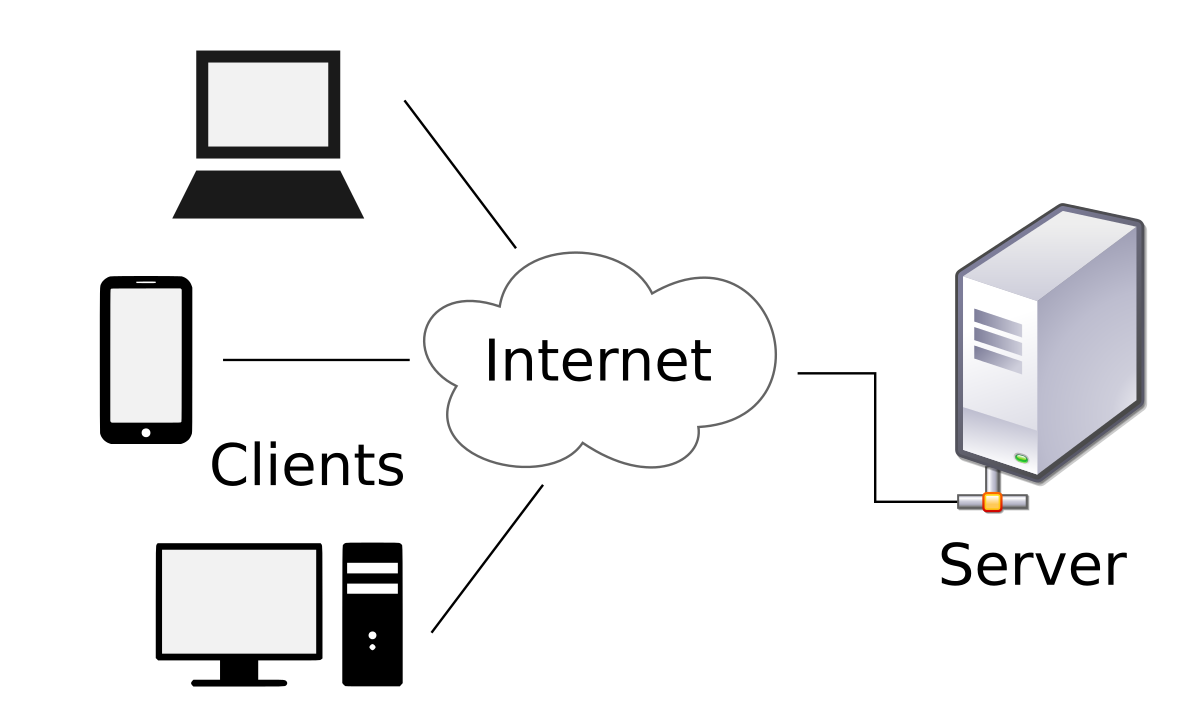
\includegraphics[width=\linewidth]{img/client-server-model.png}
		  \caption{Ilustração da arquitetura Cliente-Servidor}
		  Fonte: https://upload.wikimedia.org/wikipedia/commons/c/c9/Client-server-model.svg
		  \label{fig:client-server-model}
		\end{figure}

		\subsubsection{Vantagens e desvantagens}

			A grande vantagem e motivo principal pela escolha dessa plataforma é poder ser utilizado de qualquer dispositivo com um navegador moderno e acesso à internet. Qualquer pessoa pode acessar a solução acessando um link e começar a desenvolver e estudar códigos escritos para a arquitetura RISC-V. 
			Outra vantagem é a correção de bugs e atualizações para novas versões. Para que os usuários tenham seus softwares atualizados basta atualizar o software em um ponto apenas.

			Uma desvantagem é ter o custo de um servidor rodando a aplicação para que seja acessível por vários usuários. Outro fator crítico é ter um único ponto de falha, diferente de uma rede peer-to-peer distribuída.
			Em relação as desvantagens elas não representam uma significância alta pois se trata de uma ferramenta livre, ou seja, caso haja algum tipo de indisponibilidade do servidor, o usuário poderá baixar o software e rodar em sua própria máquina. 


		
		\subsubsection{O \textit{frontend} e o \textit{backend}}
			Podemos dividir aplicações em duas partes, o \textit{frontend} e o \textit{backend}, sendo o primeiro, a parte visual da aplicação, no caso deste projeto em específico, a parte que irá ser renderizada no navegador do usuário, HTML, CSS e JavaScripts. O segundo é o sistema com suas regras de negócio, gerências, armazenamento e recuperação de dados, entre outros.

		\subsubsection{API}

			API é uma sigla para \textit{Application Program Interface}, é uma interface de comunicação entre aplicações. Um API é definida por um conjunto de funcionalidades pré-implementadas para envio e recebimento de dados. Neste projeto utilizamos uma WEB API, com isso um servidor fornece seus serviços através de chamadas HTTP através de URLs.

			A interação entre o \textit{frontend} e o \textit{backend} é realizada por chamadas à API. Basicamente, quando um usuário clica em algum elemento interativo da aplicação, este clique envia dados ao servidor em formato \textit{JSON} e o servidor irá retornar dados no mesmo formato.

			Dessa maneira, o \textit{frontend} e o \textit{backend} funcionam de forma independente, e caso seja necessário criar um novo \textit{frontend}, por exemplo para um dispositivo diferente, ou então uma versão desktop ao invés de utilizar o navegador, é possível continuar utilizando o mesmo \textit{backend}.

